\documentclass{article}
\usepackage{pgfplots}
\usepackage{tikz-dependency}
\usepackage{graphicx}
\usepackage{subfigure}
\usepackage{tikz}
\usepackage{pgfplots}
\usepackage{times}
\usepackage{latexsym}
\usepackage[labelformat = empty]{caption}
\usepackage{floatrow}
\thispagestyle{empty}
\pgfplotsset{compat=1.9}
\usepgflibrary{arrows.meta}
\usetikzlibrary{fit}
% \renewcommand{\thesubfigure}{\alph{subfigure}}


\begin{document}

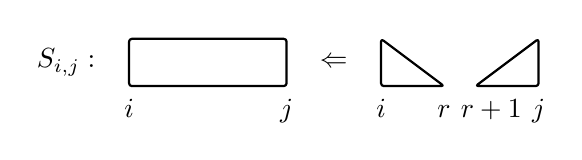
\begin{tikzpicture}[
  dep arrow/.style={
  arrows = {-Latex[round,open,length=8pt,width=6pt]},
  shorten >= 2pt,
  shorten <= 1.5pt,
  thick
  },
  dot/.style={
      inner sep=0pt,
      circle,
      draw=none
    },
  label/.style={
      anchor=base,
    },
  line/.style={
      line join=round,
      fill=none,
      % fill={rgb,255:red,76; green,114; blue,176},
      % draw={rgb,255:red,76; green,114; blue,176},
      % draw opacity=0.6,
      % fill opacity=0.1,
      rounded corners=1pt,
      thick
    }]
  \begin{scope}
    \node [dot] (i) {};
    \node [dot] (j) at ($(i) + (2.0cm, 0)$) {};

    \node [label] at ($(i) + (0, -0.4cm)$) {$i$};
    \node [label] at ($(j) + (0, -0.4cm)$) {$j$};
    \node [dot, draw=none] (j') at ($(j) + (0, 0.6cm)$) {};
    \filldraw [line] ($(i)$) -- ($(j)$) -- ($(j) + (0, 0.6cm)$) -- ($(i) + (0, 0.6cm)$) -- cycle;
    \node (placeholder_b) [draw=none, fit=(i) (j) (j')] {};
  \end{scope}

  \begin{scope}[xshift=3.2cm]
    \node [dot] (i) {};
    \node [dot] (r) at ($(i) + (0.8cm, 0)$) {};
    \node [dot] (r_1) at ($(r) + (0.4cm, 0)$) {};
    \node [dot] (j) at ($(r_1) + (0.8cm, 0)$) {};

    \node [label] at ($(i) + (0, -0.4cm)$) {$i$};
    \node [label] at ($(r) + (0, -0.4cm)$) {$r$};
    \node [label] at ($(r_1) + (0.2cm, -0.4cm)$) {$r+1$};
    \node [label] at ($(j) + (0, -0.4cm)$) {$j$};
    \node [dot, draw=none] (j') at ($(j) + (0, 0.6cm)$) {};
    \filldraw [line] ($(i)$) -- ($(r)$) -- ($(i) + (0, 0.6cm)$) -- cycle;
    \filldraw [line] ($(r_1)$) -- ($(j)$) -- ($(j) + (0, 0.6cm)$) -- cycle;
    \node (placeholder_a) [draw=none, fit=(i) (j) (j')] {};
  \end{scope}

  \node at ($(placeholder_a)!0.5!(placeholder_b)$) {$\Leftarrow$};
  \node at ($(placeholder_b) + (-1.8cm,0) $) {$S_{i, j}:$};
  % \node at ($(placeholder_b) + (-3cm,0) $) {$(\mathrm{b})$};
\end{tikzpicture}

\end{document}
